\chapter{Materials and Methods}
\label{ch:methods}

\section{Chemicals and Materials}
\label{sec:materials}
Three Spiral-wound end-of-life (EoL) RO elements were recovered from two full-scale Australian plants with different feed water and service histories (Table~ \ref{tab:membranes-source}). Two came from a seawater deesalination plant (desal site), retired after \qty{4.5}{years} of service. 4238A was a Hydranautics SWC5-LD seawater element from the first pass. 4238C was a Hydraunatics ESPA2-MAX brackish-water element from the second pass. At this site, the second-pass feed is raised to pH~$\approx$~10 to enhance boron removal, and operators reported a loss of boron rejection over service life \citep{MembraneWorks2025Desal}. 

The third, 4297B, was a Filmtec SW30XLE-440 seawater element from a mine-site water treatment plant (mine site). The plant treats a mixed-source, high-sulfate feed through \ce{KMnO4} oxidation, ultrafiltration, sodium metabisulfite dechlorination and cartridge filtration ahead of a single-stage RO system. The element was retired after \qty{2.75}{years} of service, when the salt rejection fell from approximately \qty{97}{\percent} to \qty{85}{\percent} over five weeks in early 2026.  \\


N-hexane was purchased from chem-supply, along with the monomers m-phenylenediamine (MPD, \ce{C6H4-1,3-(NH2)2}, 99\% purity) and 1,3,5-benzenetricarbonyl trichloride (TMC, \ce{C9H3Cl3O3}, $\le98\%$ purity), purchased from Sigma-Aldrich. HCl, NaOH, and EDTA were purchased for use as cleaning agents. Sodium chloride (NaCl) solutions at \qty{2000}{ppm} were prepared for solute-rejection performance tests. Milli-Q water was used throughout, and all chemicals were of analytical grade.

\begin{table}[htbp]
  \centering
  \caption{End-of-life RO elements used in this work.}
  \label{tab:membranes-source}
  \begin{tabular}{|l|l|l|l|l|}
    \hline
    Label & Site  & Model                  & Type     & Service \\
    \hline
    4238A & Desal & Hydraunatics SWC5-LD & Seawater & \qty{4.5}{y} \\
    4238C & Desal & Hydranautics ESPA2-MAX & Brackish & \qty{4.5}{y} \\
    4297B & Mine  & Filmtec SW30XLE-440    & Seawater & \qty{2.75}{y}\\
    \hline
  \end{tabular}
\end{table}

\section{Experimental design}
\label{sec:experimental-design}
The experiments were carried out in two parts/campaigns (Table~\ref{tab:campaigns}). Four main conditions were defined: as recieved (no clean, no IP), cleaned (Section~\ref{sec:cleaning}), IP without cleaning, and cleaned + IP (Section~\ref{sec:ip-method}). A fresh coupon was cut from the membrane sheet for every condition, and as such coupons were tested once across difference conditions. Coupons were tested in paids in the two-cell rig.

Campaign~1 used the two desal-site membranes, 4238A and 4238C, and covered all conditions. The no-clean conditions were run three times on the same coupon paid, but the cleaned conditions were ran only once as the supply of membrane sheet ran out. Campaign~2 then used 4238C and the mine-site element 4297B. It covered the as received, cleaned and cleaned + IP conditions with more replicates per condition. Earlier, preliminary IP-without cleaning test on 4238C is also reported. The IP protocal was identical in both campigns, however campaign~1 opted for a less intensive clean, more in-line with commercial conditions. Campaign~2 shifted to an extensive 24hr base + acid clean. All measurements are reported, including single-run conditions. Where only one value exists for a quantity, the standard deviation is not available and is reported as such. 

\begin{table}[htbp]
  \centering
  \caption{Experimental campaigns and number of coupons per condition.}
  \label{tab:campaigns}
  \begin{tabular}{llcccc}
    \toprule
    Campaign & Element & As received & Cleaned & IP (no clean) & Cleaned + IP \\
    \midrule
    1 & 4238A (desal, 1st pass) & 2 (3 runs) & 2 (1 run) & 2 (3 runs) & 2 (1 run) \\
    1 & 4238C (desal, 2nd pass) & 2 (3 runs) & 2 (1 run) & 2 (3 runs) & 2 (1 run) \\
    2 & 4238C (desal, 2nd pass) & 4 & 7 & 2\textsuperscript{a} & 4 \\
    2 & 4297B (mine)            & 4 & 6 & --- & 2 \\
    \bottomrule
  \end{tabular}
  \par\smallskip
  \footnotesize \textsuperscript{a}Preliminary test, PWP and rejection only.
\end{table}

\begin{figure}[htbp]
  \centering
  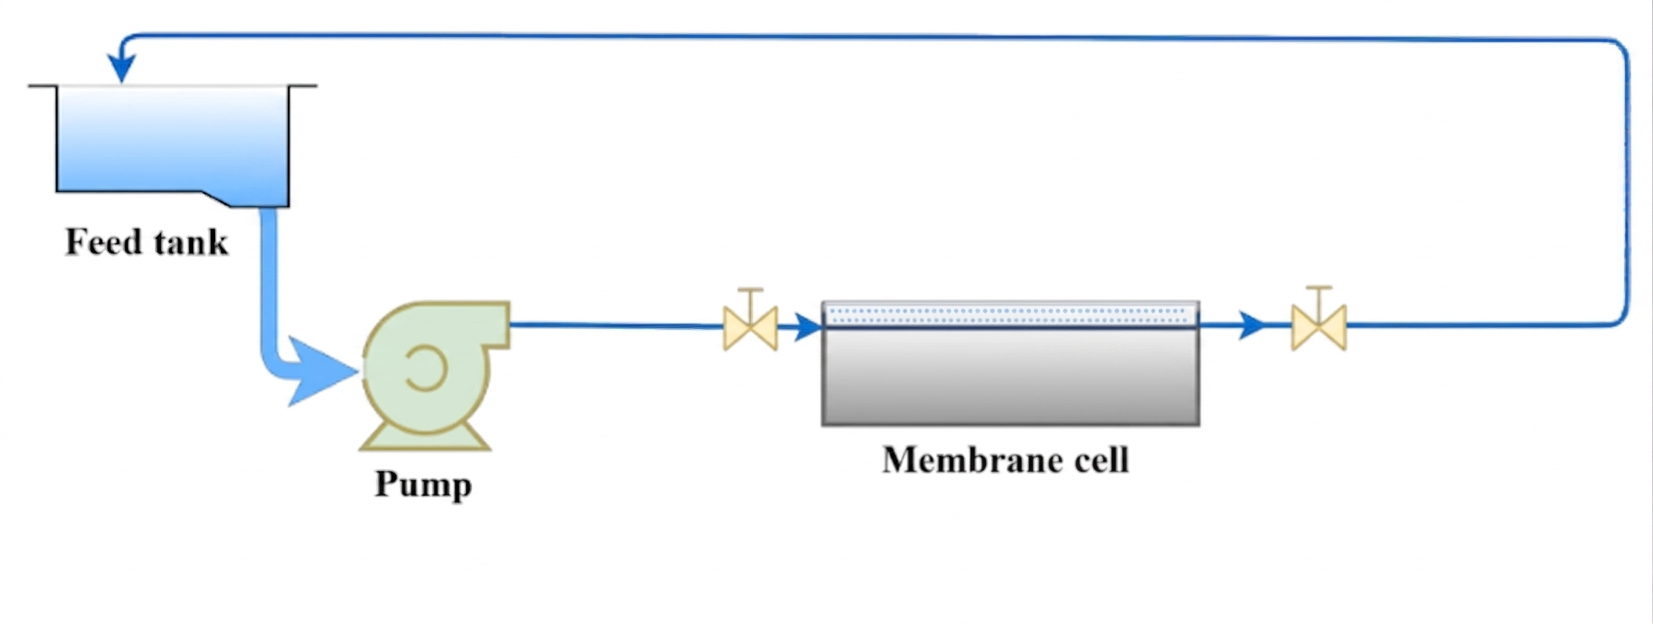
\includegraphics[width=0.8\textwidth]{figures/IP_Setup_Diagram.jpg}
  \caption{Schematic of the interfacial polymerisation setup.}
  \label{fig:ip-setup}
\end{figure}

\section{Fouling characterisation of the as-received membranes}
\label{sec:fouling-characterisation}
The condition of each element before cleaning was established by autopsy at Membrane Works Pty Ltd. The two desal-site elements (4238A and 4238C) were autopsied together, alongside unused elements of the same models (4238B and 4238D) \citep{MembraneWorks2025Desal}. The mine-site element was autopsied separately \citep{MembraneWorks2026Mine}. The techniques applied are listed in Table~\ref{tab:autopsy-coverage}.

\begin{table}[htbp]
  \centering
  \caption{Autopsy techniques applied to each element.}
  \label{tab:autopsy-coverage}
  \begin{tabular}{lccc}
    \toprule
    Technique                                  &4238A & 4238C      & 4297B      \\
    \midrule
    Vacuum decay integrity test                & ---       & ---        & \checkmark \\
    External and internal visual inspection    & \checkmark & \checkmark & \checkmark \\
    Standardised flux and salt rejection       & \checkmark & \checkmark & ---        \\
    Dye penetration test                       & \checkmark & \checkmark & ---        \\
    Optical microscopy and Astra Blue staining & ---        & ---        & \checkmark \\
    SEM-EDS                                    & \checkmark & \checkmark & \checkmark \\
    ATR-FTIR                                   & \checkmark & \checkmark & ---        \\
    Zeta potential and isoelectric point       & \checkmark & \checkmark & ---        \\
    Water contact angle                        & \checkmark & \checkmark & ---        \\
    Acid/caustic extractable analysis          & ---        & ---        & \checkmark \\
    Total viable count                         & ---        & ---        & \checkmark \\
    Fujiwara test                              & ---        & ---        & \checkmark \\
    XPS                                        & ---        & ---        & \checkmark \\
    \bottomrule
  \end{tabular}
\end{table}

\paragraph{Visual inspection.}
All elements were inspected externally including the end caps, brine seals and permeate tubes which was swabbed for deposits as an indicator of integrity breach. Each element was cut open and unrolled, and the feed side, spacer and permeate were examined for colour, texture and odour, as well as delamination, compaction and physical damage. 

\paragraph{Performance and dye penetration.}
The performance of the 4238A and 4238C was measured on in-situ test rig using the manufacturer's conditions of (\qty{1500}{mg.L^{-1}} NaCl, \qty{10.3}{bar}, \qty{25}{\celsius}, \qty{15}{\percent} recovery, pH~7). Flux and rejection were calculated (from conductivity) and compared against the unused membrane element. The membrane coupon were then subjected to dye-testing with \qty{10}{mg.L^{-1}} methyl violet under pressure in a static flat-sheet cell. The permeate side was inspected for dye passage through PA defects. 

\paragraph{Surface characterisation.}
Surface characterisation of the as-received elements was carried out by Membrane Works as part of the autopsie. SEM-EDS and ATR-FTIR were the main techniques used for this characterisation. 

\flag{SEM-EDS}

ATR-FTIR was used to detect chemical change in the membrane surface. Spectra of 4238A and 4238C were compared against the unused reference element 4238B and 4238D respectively. The sampling depth allows both the PA and PSf to be captured. The state of PA layer was judged by the amide carbonyl (C=O) strengthing band near \qty{1663}{cm^{-1}}, the dominant PA signiture. Additionally, the support-layer bands \qty{1585}{} and \qty{1243}{cm^{-1}}, and the broad O--H/N--H stretching band centred near \qty{3336}{cm^{-1}} reflects carboxylic acid and amide groups \citep{Ogbe2025}. These bands can indicate the loss or degradatino of the PA layer. 


\section{Chemical cleaning protocol}
\label{sec:cleaning}
The EoL membranes were chemically cleaned before IP so that the new polyamide layer would form on the existing active layer rather than on deposited foulant, allowing cleaned and uncleaned coupons to be compared. The autopsies showed mixed fouling of organic and biological material, calcium and magnesium salts, and metal oxides (Section~\ref{sec:res-fouling}), so a two-step clean was used: an alkaline clean with EDTA to remove organic and biological foulants and chelate divalent cations, followed by an acid clean to dissolve the remaining inorganic scale (Section~\ref{sec:lit-cleaning}).

Two cleaning protocols were used. For the first campaign, coupons 4238A and C received a commercial clean, which involves a 1 hour soak used for routine cleaning of fouled elements in industry \citep{DuPont2026, Lenntech2011}. Campaign 2 coupons (4238C and 4297B) received an extensive clean with the same alkaline-acid sequence but with higher chemical doses, continuous stirring and 24 hour soaks. The aim was to remove stubborn fouling on the EoL elements. Apart from the parameters in Table \ref{tab:cleaning-protocols}, both protocols followed the same procedure (Section \ref{sec:cleaning-procedure}).

\begin{table}[htbp]
  \centering
  \caption{Commercial (Campaign~1) and extensive (Campaign~2) cleaning parameters. All other steps were identical (Section~\ref{sec:cleaning-procedure}).}
  \label{tab:cleaning-protocols}
  \begin{tabular}{lll}
    \toprule
    Parameter & Commercial clean & Extensive clean \\
    \midrule
    Solution volume per sheet & 1~L & 1.5~L \\
    Agitation & None (static soak) & Magnetic stirrer, 100~rpm \\
    \midrule
    \multicolumn{3}{l}{\textit{Alkaline clean}} \\
    NaOH & 0.1\% w/v (2.0~g per 2~L) & 0.23\% w/v (3.50~g per 1.5~L) \\
    Na-EDTA & 0.5\% w/v (10~g per 2~L) & 1.0\% w/v (15~g per 1.5~L) \\
    Measured pH & 10.6 & 11.14--11.58 \\
    Soak time & 1~h & 24~h \\
    \midrule
    Intermediate rinse & \multicolumn{2}{l}{10~min, continuous RO water} \\
    \midrule
    \multicolumn{3}{l}{\textit{Acid clean}} \\
    HCl (32\% w/w) & 7~mL per 2~L ($\approx$0.13\% w/v) & 15~mL per 1.5~L ($\approx$0.37\% w/v) \\
    Measured pH & 1.6 & 1.4 \\
    Soak time & 1~h & 24~h \\
    \midrule
    Final rinse & \multicolumn{2}{l}{Continuous RO water until free of cleaning agents} \\
    \bottomrule
  \end{tabular}
\end{table}

All cleaning was performed ex-situ by soaking at room temperature (approximately \SI{22}{\celsius}), above the minimum effective cleaning temperature of \SI{20}{\celsius} \citep{Lenntech2011}. Membrane sheets were cleaned separately, cut into rectangles of around \qty{350}{\square\centi\metre} and solutions were prepared with Milli-Q water. Solution pH was measured with a calibrated pH meter after each solution was prepared. 

\subsection{Commercial clean}
\label{sec:com-cleaning}
The commercial cleaning followed routine industrial practice. Membrane sheets were laid flat in clear dishes and soaked statically in 1L of solution for 1h per chemical \citep{DuPont2026}. The alkaline solution contained \qty{0.1}{\percent} w/v NaOH and \qty{0.5}{\percent} w/v Na-EDTA, giving pH 10.6. This matches the pH $\approx$10.5 used industrially for a \qty{0.1}{\percent} NaOH clean \citep{zwaneveld2026personal}, but is below the pH 11 reported to optimise the deprotonation of foulant group carboxylic groups \citep{Ang2006}. The acid solution (7 mL of \qty{32}{\percent} w/w HCl in 2L) gave pH 1.6, within the pH 1-2 range specified by \cite{DuPont2026}. 

\subsection{Extensive clean}
\label{sec:ext-cleaning}
Because the membrane tested are EoL elements with consolidated fouling layers, the commercial protocol was modified:
\begin{itemize}
\item Extended contact time: each chemical step was run for 24 h rather than 1 h. \cite{DuPont2026} recommends an overnight soak of 10–15 h for difficult fouling; extending to 24 h ensures that contact time does not limit foulant removal.
\item Continuous agitation: solutions were stirred with a magnetic stirrer at 100 rpm throughout each soak. Industrial cleaning recirculates solution through the element, and low-speed stirring gives better mass transfer than a static soak.
\item Higher chemical doses: EDTA was raised to \qty{1.0}{\percent} w/v, consistent with the \qty{1}{\percent} specified by \cite{DuPont2026} and the \qty{0.8}{\percent} given by \cite{Lenntech2011}. NaOH was raised to \qty{0.23}{\percent} w/v because the disodium EDTA salt consumes part of the caustic, as shown by the commercial clean, which reached only pH 10.6 at \qty{0.1}{\percent} NaOH. The resulting pH of 11.14–11.58 across batches sits around the pH 11 optimum of \cite{Ang2006}, within the pH 10–11.5 window of \cite{Lenntech2011} and within the pH 1–13 tolerance of polyamide membranes at $\le$ \SI{25}{\celsius} \citep{DuPont2026}. The acid dose was raised to 15 mL of \qty{32}{\percent} HCl per 1.5 L, giving pH 1.4, still within the pH 1–2 range of \cite{DuPont2026}.
\end{itemize}

\subsection{Cleaning Procedure}
\label{sec:cleaning-procedure}
\subsubsection*{Alkaline (caustic) clean with chelant}

\begin{enumerate}

\item The membrane sheet was cut to size (\qty{30}{\centi\metre} × \qty{10}{\centi\metre} for the extensive clean).

\item The required volume of Milli-Q water was measured out. NaOH pellets were weighed and dissolved in a portion of this water with manual stirring until fully dissolved.

\item Na-EDTA was weighed and dissolved into the same solution.

\item The pH of the combined solution was measured and recorded.

\item The membrane sheet was fully submerged in the alkaline solution and soaked at room temperature without heating for the specified time. In the extensive clean, the vessel was covered with aluminium foil and stirred at 100 rpm.

\end{enumerate}

\subsubsection*{Intermediate rinse}

\begin{enumerate}[resume]

\item Following the alkaline soak, the membrane was rinsed continuously with RO water for 10 min to remove residual alkaline solution, which would otherwise neutralise the acid solution on contact.

\end{enumerate}

\subsubsection*{Acid clean}

\begin{enumerate}[resume]

\item \qty{32}{\percent} w/w HCl was added to Milli-Q water and mixed.

\item Solution pH was measured and recorded.

\item The membrane sheet was fully submerged in the acid solution and soaked at room temperature without heating for the specified time, covered and stirred at 100 rpm in the extensive clean.

\end{enumerate}

\subsubsection*{Final rinse}

\begin{enumerate}[resume]

\item The membrane was rinsed continuously with RO water until free of cleaning agents.

\end{enumerate}


\section{In-situ interfacial polymerisation}
\label{sec:ip-method}

In-situ IP was performed in a custom flat-sheet crossflow system using a dry acrylic membrane cell (\qtyproduct{280 x 125 x 50}{\milli\metre}) that exposed the active surface of the membrane sheet. A peristaltic pump circulated solution at \qty{1.5}{\litre\per\minute} to maintain consistent mass transfer, with the cell outlet returning liquid to the feed tank. For curing, the liquid feed was replaced with heated air: compressed air passed through a stainless steel coil submerged in a temperature-controlled water bath, and a downstream temperature sensor verified that air reached the cell at the target curing temperature. Regulating both air temperature and flow rate to the cell enabled controlled and uniform curing of the PA layer.

EoL RO membranes were mounted in the acrylic cell and an aqueous MPD phase (\qty{3.75}{\gram} in \qty{250}{\milli\litre}) was circulated at \qty{1.5}{\litre\per\minute} for \qty{3}{\minute}. The membrane was then removedfrom the cell and dried, before the organic TMC/hexane phase(\qty{330}{\micro\litre} in \qty{250}{\milli\litre}) was circulated for \qty{1}{\minute}. Curing followed at \qty{60}{\degreeCelsius} and \qty{10}{\litre\per\minute} for \qty{5}{\minute}.

The same monomer concentrations, contact times and curing conditions were used for every IP run in both campaigns.

\section{Membrane Performance test using High-pressure crossflow rig and compaction}
\label{sec:rig performance}
Membrane performance was evaluated in terms of pure water permeability (PWP) and salt rejection, using a high-pressure crossflow rig that holds two flat-sheet membranes in parallel cells, each with an effective area of \qty{0.0139}{\metre\squared}. Applied pressure was logged through CIMPLICITY software. Feed temperature was held at \qty{25}{\degreeCelsius}

Permeate was collected in a pre-weighted container over a timed interval and weighed on an analytical balance. Volume was then obtained from mass assuming a water density of \qty{0.997}{\gram\per\milli\litre} at \qty{25}{\degreeCelsius}. Collection began after \qty{10}{\minute} stabilisation period. 

\subsection{Compaction}
Before testing, each coupon was compacted with pure water at \qty{15}{bar} for at least \qty{30}{\minute}. This reduces the flux decline caused by compression of porous support so measurements taken reflect a stable membrane structure. After this period, flux was generally observed to be stable with $<5\%$ change over the experiment timeframe. 

\subsection{Pure Water Permeability}
PWP was measured with deionised water so no osmotic pressure opposes the flow. Water flux was calculated as
\begin{equation}
  J_w = \frac{\Delta V}{A_m\,\Delta t}
  \label{eq:water-flux-methods}
\end{equation}
Here $\Delta V/\Delta t$ is the permeate volume collected per unit time.  $A_m$ is the effective membrane area of $\SI{0.0139}{\square\metre}$. PWP is then obtained by normalising the flux by the transmembrane pressure $\Delta P$: 

\begin{equation}
  A = \frac{J_w}{\Delta P},
  \label{eq:pwp-methods}
\end{equation}

Flux is reported in L\,m$^{-2}$\,h$^{-1}$ (LMH) and PWP in LMH\,bar$^{-1}$. Each coupon had PWP measured in triplicate.


\subsection{Salt Rejection}
Salt rejection was measured with a \qty{2000}{ppm} NaCl feed at pH~$7.0 \pm 0.2$ and \qty{25}{\degreeCelsius}. This corresponds to a feed conductivity of approximately \qty{3.7}{} to \qty{4.0}{\milli\siemens\per\centi\metre}. Feed and permeate conductivities were measured with a TPS WP-81 conductivity/pH meter, fitted with a conductivity sensor with automatic temperature compensation. Feed conductivity was taken as the mean of three to four readings from feed tank. Observed rejection was calculated as

\begin{equation}
  R = \left(1 - \frac{C_p}{C_f}\right) \times 100\%,
  \label{eq:rejection-methods}
\end{equation}

Here $C_p$ and $C_f$ is the permeate and bulk feed concentration. Conductivity is assumed to be proportional to the NaCl concentration so conductivities were used directly in place of concentration. Permeate volume is small compared to feed tank (3L) so recovery is negligible and feed tank concentration was taken as the bulk feed concentration. Three repeated readings were taken from each permeate samples and the average was calculated. 

\subsection{Salt Permeability and Selectivity}
Observed rejection depends on water flux as well as on the membrane (Section-\ref{sec:Performance-Characterisation}). The apparent solute transport parameter, $B$, was then calculated for each coupon from the salt-test flux and rejection:
\begin{equation}
  B = J_w\,\frac{1 - R}{R}
  \label{eq:b-methods}
\end{equation}



\section{Post-regeneration membrane autopsy}
\label{sec:autopsy}
Coupons were characterised after cleaning and after interfacial polymerisation, following protocols of \cite{Ogbe2025}. Before analysis, coupons were dried at \qty{30}{\celsius} for \qty{1}{h} so that residual water would not interfere with the measurements

\paragraph{ATR-FTIR}
Surface chemistry was analysed by ATR-FTIR on a Bruker Alpha~II spectrometer with OPUS softwar. Each spectrum was the average of 32 scans over \qtyrange{400}{4000}{cm^{-1}} at \qty{4}{cm^{-1}} resolution \citep{Ogbe2025}. Spectra was compared against the EoL baseline.  

\paragraph{SEM}
Surface morphology was examined by SEM at the Mark Wainwrite Analytical Centre, UNSW. Micrographs were used as a qualitative record of the state of the PA layer. An intact RO active layer would show in images as a ride and valley structure. The loss of PA layer would show a smoother surface in which the pores of the support layer would be visible. 


\section{Data treatment and statistical analysis}
\label{sec:stats}
Repeat readings on coupons were first averaged to give coupon mean. For each element and condition, results are reported as the mean $\pm$ sample standard deviation (SD) of the coupon means, with $n$ the number of coupons. Where 95\,\% confidence intervals are given, they are $\bar{x}\pm t_{0.975, \, n-1}\,s/\sqrt{n}$. 

Because fresh coupons were used for every condition rather than the same coupon tested, altered then tested again, they were treated as independent groups using Welch's two-sample $t$-test, which does not assume equal variance. Each comparison reports difference in means with its 95\,\% confidence interval and the $p$-value. Differences are described as significant at $\alpha = 0.05$. Campaign~1 and Campaign~2 were analysed separately. Data were compiled in Excel, and the statistics were calculated in Python (pandas, SciPy).
